% author: Naijia Liu
% resource for the latex template: https://www.overleaf.com/latex/templates/uq-beamerposter-template/svbpbndqdpqv
% please refer to https://www.overleaf.com/learn for more information and instructions
% We are generating "Air Quality Forecast and Dispersion Outlook of Allegheny County, Pennsylvania" report using Latex


% define the document class for the report: beamer
% this can be useful if you find some latex grammar is not working
% try to google your problem like "problem + beamer + latex"
\documentclass[final, xcolor=table]{beamer}

% ====================
% Packages
% ====================

% please put the logos and the pictures used in the report
% in the "logos" file of the Github repository

\usepackage[T1]{fontenc}
\usepackage{lmodern}
\usepackage[size=custom,width=100,height=75,scale=1.0]{beamerposter}
\usetheme{gemini}
\usecolortheme{uchicago}
\usepackage{graphicx}
\usepackage{booktabs}
\usepackage{tikz}
\usepackage{pgfplots}
\pgfplotsset{compat=1.17}
\usepackage{tabularx}
\usepackage{adjustbox}
\usepackage{hyperref}
\definecolor{mycolor}{HTML}{000AFC}
\hypersetup{
    colorlinks=true,
    urlcolor=mycolor
    }
    
% data input from the data_X07 file

\newcommand\AQIPittToday{41}
\newcommand\AQIPittTom{52}
\newcommand\AQILCToday{38}
\newcommand\AQILCTom{55}
\newcommand\AQIPittTodayCate{Good}
\newcommand\AQIPittTomCate{Moderate}
\newcommand\AQILCTodayCate{Good}
\newcommand\AQILCTomCate{Moderate}
\newcommand\AQIpitttodaypolutant{PM 2.5}
\newcommand\AQIpitttomorrowpolutant{PM 2.5}
\newcommand\AQILCtodaypolutant{PM 2.5}
\newcommand\AQILCtomorrowpolutant{PM 2.5}
\newcommand\Discriptions{Current Conditions as of 2 PM on Monday:Rain showers associated with the remnants of once Hurricane Ian have stayed to the east on Monday.Some higher clouds are pushing westward into the region this afternoon, but conditions should remain dry.*** Tuesday's Forecast:With the remnants of once Hurricane Ian to the east and high pressure to the west, the flow will remain northerly on Tuesday.Temperatures will climb into the low to mid-60s under a mix of sun and clouds.Concentrations of fine particulate matter (PM-2.5) will remain at levels inside the good range for the day.}
\newcommand\ADIone{Fair - 29}
\newcommand\ADItwo{Generally Good - 55}
\newcommand\ADIthree{Very Poor - 2}
\newcommand\ADIfour{Very Poor - 2}
\newcommand\ADIfive{Very Poor - 5}
\newcommand\ADIsix{Generally Poor - 20}
\newcommand\SISone{None}
\newcommand\SIStwo{--}
\newcommand\SISthree{--}
\newcommand\SISfour{--}
\newcommand\SISfive{None}
\newcommand\SISsix{--}
\newcommand\Windone{N - 6}
\newcommand\Windtwo{N - 7}
\newcommand\Windthree{N - 3}
\newcommand\Windfour{NW - 5}
\newcommand\Windfive{N - 5}
\newcommand\Windsix{NW - 6}
\newcommand\Temp{0 °C}
\newcommand\Depth{0 m}
\newcommand\Time{--}
\newcommand\Scale{None}
\newcommand\Inversion{No upper inversion starting below ~1000 m is reported}
\newcommand\Title{Air Quality Forecast and Dispersion Outlook \\of Allegheny County, Pennsylvania for 2022-10-04}
\newcommand\AQIPittTodayColor{6AFE19}
\newcommand\AQIPittTomColor{FFF421}
\newcommand\AQILCTodayColor{6AFE19}
\newcommand\AQILCTomColor{FFF421}
\newcommand\AQIDateToday{10/04/2022}
\newcommand\AQIDateTom{10/05/2022}
\newcommand\AQIWeekToday{Tuesday}
\newcommand\AQIWeekTom{Wednesday}
\newcommand\inversionmode{observation}


% ====================
% Lengths
% ====================

% If you have N columns, choose \sepwidth and \colwidth such that
% (N+1)*\sepwidth + N*\colwidth = \paperwidth
% there are 2 columns in the report
\newlength{\sepwidth}
\newlength{\colwidth}
\setlength{\sepwidth}{0.03\paperwidth}
\setlength{\colwidth}{0.45\paperwidth}

% define the layout for the report
\newcommand{\separatorcolumn}{\begin{column}{\sepwidth}\end{column}}

% ====================
% Title
% ====================

% extract title using the date we generated
\title{\Title}

\author{Allegheny County Health Department}

% this is the invisible line that is under the "Allegheny County Health Department"
% we are not exactly using this line of code
% !!DO NOT DELETE IT!!
% or the code will report an error
\institute[shortinst]{ \samelineand }

% ====================
% Footer (optional)
% ====================

\footercontent{
  \href{https://www.alleghenycounty.us/Health-Department/Programs/Air-Quality/Air-Quality.aspx}{\color{white}{https://www.alleghenycounty.us/Health-Department/Programs/Air-Quality/Air-Quality.aspx}} \hfill
  Allegheny County \hfill
  412-687-2243}
% (can be left out to remove footer)

% ====================
% Logo (optional)
% ====================

% use this to include logos on the left and/or right side of the header:
% \logoright{\includegraphics[height=7cm]{logo1.pdf}}
% \logoleft{\includegraphics[height=7cm]{logo2.pdf}}

% ====================
% Body
% ====================

\begin{document}
% include the logos on the left and right of the headline
\addtobeamertemplate{headline}{}
{
    \begin{tikzpicture}[remember picture,overlay]
      \node [anchor=north west, inner sep=3.5cm] at ([xshift=-2cm,yshift=2.5cm]current page.north west)
      {
\includegraphics[height=2.6cm]{logos/allegheny.png}}; % also try shield-white.eps
      \node [anchor=north east, inner sep=3cm] at ([xshift=0.0cm,yshift=1.5cm]current page.north east)
      {
\includegraphics[height=8.0cm]{logos/achd.png}};
    \end{tikzpicture}
}
% you can adjust the position of the logo using "xshift" and "yshift"
% use "height" to adjust the size of the picture


\begin{frame}[t]
\begin{columns}[t]
\separatorcolumn

% =============
% Left Column
% =============

\begin{column}{\colwidth}

% ========================================
% First block of  "Air Quality Forecast"
% ========================================

  \begin{block}{Air Quality Forecast} % block name
    This is the daily forecasted Air Quality Index (AQI) for each area provided by the PA Department of Environmental Protection. The AQI is based on PM2.5 or Ozone, whichever is forecasted to be higher.
   
    % the functions these tables uses
    % \rowcolor[HTML]{"include the words here"}: the color of the entire row using the html code for the color
    % \cellcolor[HTML]{"include the words here"}: the color of the cell using the html code for the color
    % \textbf{}: bold the words
    % \multicolumn{}: create multi-column in the table
    
    
    \begin{table}
      \renewcommand{\arraystretch}{1.5} % use to adjust the height of all the rows
      \centering
      \begin{tabular}{|c| c| c|} % 3 columns for the table
        \hline
        \rowcolor{lightgray}\textbf{Forecast Period} & \textbf{Pittsburgh Area} & \textbf{Liberty-Clairton Area} \\ % line break
        \hline
        \rowcolor[HTML]{F2FDFE} {\textbf{Today}} &  {\cellcolor[HTML]{\AQIPittTodayColor}PM2.5} & {\cellcolor[HTML]{\AQILCTodayColor}PM2.5}\\ 
        
        \rowcolor[HTML]{F2FDFE} {\AQIWeekToday} & {\cellcolor[HTML]{\AQIPittTodayColor}\textbf{\AQIPittTodayCate}} & {\cellcolor[HTML]{\AQILCTodayColor}\textbf{\AQILCTodayCate}} \\
        
        \rowcolor[HTML]{F2FDFE} {\AQIDateToday} & {\cellcolor[HTML]{\AQIPittTodayColor}{\AQIPittToday} AQI} & {\cellcolor[HTML]{\AQILCTodayColor}{\AQILCToday} AQI} \\
        
        \hline
        % include "hline" when you want to draw an actual
        % border for the above row inside the table
        
        \rowcolor[HTML]{F2FDFE} {\textbf{Tomorrow}} & {\cellcolor[HTML]{\AQIPittTomColor}PM2.5} & {\cellcolor[HTML]{\AQILCTomColor}PM2.5}\\ 
        
        \rowcolor[HTML]{F2FDFE} {\AQIWeekTom} & {\cellcolor[HTML]{\AQIPittTomColor}\textbf{\AQIPittTomCate}} & {\cellcolor[HTML]{\AQILCTomColor}\textbf{\AQILCTomCate}} \\
        
        \rowcolor[HTML]{F2FDFE} {\AQIDateTom}& {\cellcolor[HTML]{\AQIPittTomColor}{\AQIPittTom} AQI} & {\cellcolor[HTML]{\AQILCTomColor}{\AQILCTom} AQI} \\
        
        \hline
      \end{tabular}
      \caption{Please refer the Air Quality Index guide}
    \end{table}

    % forecast section
    \heading{Today’s Forecast:}
    \Discriptions
    

    \begin{table}
      \begin{adjustbox}{width=1\textwidth}
      \renewcommand{\arraystretch}{1.5}
      \centering
      \begin{tabular}{|c |c |c |c|}
      \hline
      \rowcolor{lightgray}\multicolumn{4}{|c|}{\textbf{Guide to the Air Quality Index (AQI)}} \\
      \hline
      \rowcolor{lightgray}\textbf{Color} & \textbf{Description} & \textbf{Meaning} & \textbf{AQI} \\
      \hline
      \rowcolor[HTML]{F2FDFE}{\cellcolor[HTML]{FF2121}\textbf{Red}} & Unhealthy & Everyone should limit exertion outdoors. & 151 - 200 \\
      \rowcolor[HTML]{F2FDFE}{\cellcolor[HTML]{FF6A20}\textbf{Orange}} & Unhealthy for Sensitive Groups & Sensitive people should limit exertion outdoors. & 101 - 150 \\
      \rowcolor[HTML]{F2FDFE}{\cellcolor[HTML]{FFF421}\textbf{Yellow}} & Moderate & Extremely sensitive people may wish to limit outdoor exertion. & 51 - 100 \\
      \rowcolor[HTML]{F2FDFE}{\cellcolor[HTML]{6AFE19}\textbf{Green}} & Good & No health impacts are expected in this range. & 0 - 50 \\
      \hline
      \end{tabular}
      \end{adjustbox}
    \end{table}

    \href{https://www.ahs.dep.pa.gov/AQPartnersWeb/forecast_home.aspx}{\underline{Data provided by the PA Department of Environmental Protection}}

  \end{block} 
  % here, we end the first block of  "Air Quality Forecast"
  
% ============================================================
% Second block of "ACHD Surface Temperature Inversion Report"
% ============================================================

  \begin{block}{ACHD Surface Temperature Inversion Report}

    \textit{This is the 7 AM surface-based temperature inversion report for Allegheny County.}

    % first line of inversion report
    This morning’s surface inversion of \underline{\textbf{$\sim$\Temp}} with a depth of \underline{\textbf{$\sim$\Depth}} is estimated to break at \underline{\textbf{\Time}}. 
    
    % second line of inversion report
    This surface inversion can be characterized as: \underline{\textbf{\Scale}} (None / Slight / Weak / Moderate / Strong. 
    
    % third line of inversion report
    \Inversion

  \end{block}
  % here, we end the second block

\end{column} 
% here, we end the left column

\separatorcolumn
% use this to separate between columns


% =============
% Right Column
% =============

\begin{column}{\colwidth}

% =======================================================
% Third block of "ACHD Air Dispersion 36-Hour Forecast"
% =======================================================

  \begin{block}{ACHD Air Dispersion 36-Hour Forecast}

    This is the dispersion forecast for Allegheny County starting from this morning through tomorrow afternoon. The atmospheric dispersion index is a rating of the atmosphere’s ability to transport pollution away from its source and is based on emissions and weather. Better atmospheric dispersion can improve air quality.

    \begin{table}
      \renewcommand{\arraystretch}{1.5}
      \centering
      \begin{adjustbox}{width=1\textwidth}
      \begin{tabular}{ |c|c|c|c|c|}
          \hline
          \rowcolor{lightgray}\multicolumn{2}{|c|}{\textbf{Forecast Period}} & \textbf{Atmospheric Dispersion Index} & \textbf{Surface Inversion Strength} & \textbf{Wind (dir, mph)}\\
          \hline
          \rowcolor[HTML]{F2FDFE}{\textbf{Today}} & Morning & \ADIone & \SISone & \Windone \\ 
          \rowcolor[HTML]{F2FDFE} & Afternoon & \ADItwo & \SIStwo & \Windtwo \\
          \hline
          \rowcolor[HTML]{F2FDFE}{\textbf{Tonight}} & Evening  & \ADIthree & \SISthree & \Windthree\\
          \rowcolor[HTML]{F2FDFE} & Overnight & \ADIfour & \SISfour & \Windfive\\
          \hline
          \rowcolor[HTML]{F2FDFE}{\textbf{Tomorrow}} & Morning & \ADIfive & \SISfive & \Windfive\\
          \rowcolor[HTML]{F2FDFE} & Afternoon & \ADIsix & \SISsix & \Windsix\\
          \hline
      \end{tabular}
      \end{adjustbox}
      \caption{Please refer the Atmospheric Dispersion Index guide and the daily Surface Temperature Inversion Report.}
    \end{table}

    \heading{ACHD Remarks:}
    Chance of rain this morning and rain likely tomorrow. Also, the sounding data from the National Weather Service was unavailable, so I had to use an alternative source.
    
    Data provided by the National Weather Service (NWS)
    \href{https://forecast.weather.gov/product.php?site=NWS&product=FWF&issuedby=PBZ}{\underline{Fire Weather Planning Forecast}} and \href{http://weather.uwyo.edu/upperair/sounding.html}{\underline{PIT NWS Products}} 
    % include the hyper link:
    %\href{"link for the website"}{\underline{"show the word/sentence"}}
    % use \url{} command to display the actual link
    
    
    \begin{table}
      \renewcommand{\arraystretch}{1.5}
      \centering
        \begin{tabular}{ |c |c |c |c|c |c |c|  }
        \hline
        \rowcolor{lightgray}\multicolumn{7}{|c|}{\textbf{Guide to the Atmospheric Dispersion Index}} \\
        \hline
        \rowcolor[HTML]{F2FDFE}\textbf{Very Poor} & \textbf{Poor} & \textbf{Generally Poor} & \textbf{Fair} & \textbf{Generally Good} & \textbf{Good} & \textbf{Very Good} \\
        \hline
        \rowcolor[HTML]{F2FDFE}1 - 6 & 7 - 12 & 13 - 20 & 21 - 40 & 41 - 60 & 61 - 100 & > 100 \\
        \hline
        \end{tabular}
    \end{table}

  \end{block}


% =========================================================================
% Forth block of "What does the Surface Temperature Inversion Report mean"
% =========================================================================

  \begin{block}{What does the Surface Temperature Inversion Report mean}

    A surface temperature inversion is a weather pattern that stops mixing of the air near the ground, and pollution released into the air tends to remain at higher concentrations.
    
    % here, we divide this block into 2 columns
    \begin{columns}[T]
    
        % the left column for the picture
        \begin{column}{0.43\linewidth}
        
        ~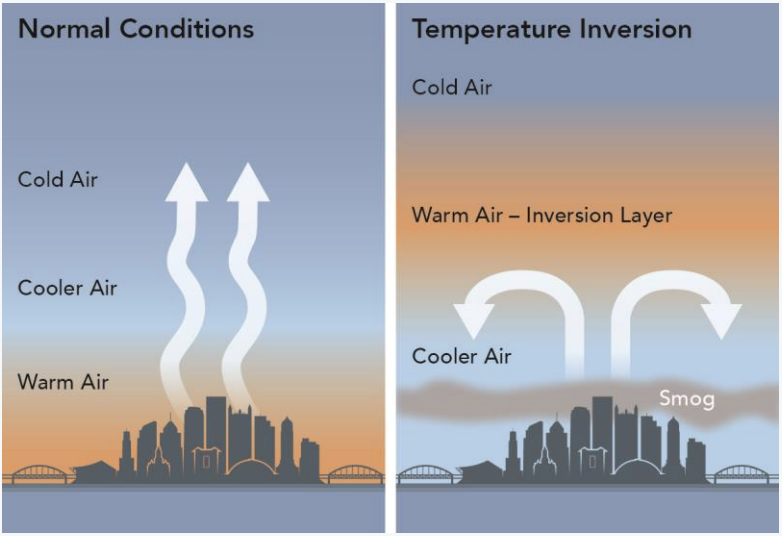
\includegraphics[width=1\textwidth]{citypic.png}
        
        \end{column}
        
        % the right column for the paragraph
        \begin{column}{0.5\linewidth}
        
            Surface temperature inversion conditions include how strong the surface inversion is (in °C), how high the inversion is above the surface (in meters), and when the inversion is expected to break (in Eastern Standard Time). Also included is whether an upperlevel inversion or inversions exist, starting at about 1,000 meters.
            
            \textbf{Surface Temperature Inversion Characterization}
                % use itemize for the list
                \begin{itemize}
                  \item 0-0.9 C°: Slight
                  \item 1-2.9 C°: Weak
                  \item 3-4.9 C°: Moderate
                  \item ≥5 C°: Strong
                \end{itemize}
        \end{column}
    
    \end{columns}    


  \end{block}


\end{column}

\separatorcolumn
\end{columns}
\end{frame}
\end{document}







